\documentclass[tikz]{standalone}

\usepackage{pgfplots}
\usetikzlibrary{calc,positioning}
\pgfplotsset{compat=newest, scale only axis, width = 10cm}
\pgfplotsset{sciclean/.style={axis lines=left,
        axis x line shift=0.5em,
        axis y line shift=0.5em,
        axis line style={-,very thin},
        axis background/.style={draw,ultra thin,gray},
        tick align=outside,
        xtick distance=1,
        ytick distance=1,
        major tick length=2pt}}

% Create fake \onslide and other commands for standalone picture
\usepackage{xparse}
\NewDocumentCommand{\onslide}{s t+ d<>}{}
\NewDocumentCommand{\only}{d<>}{}
\NewDocumentCommand{\uncover}{d<>}{}
\NewDocumentCommand{\visible}{d<>}{}
\NewDocumentCommand{\invisible}{d<>}{}

\begin{document}

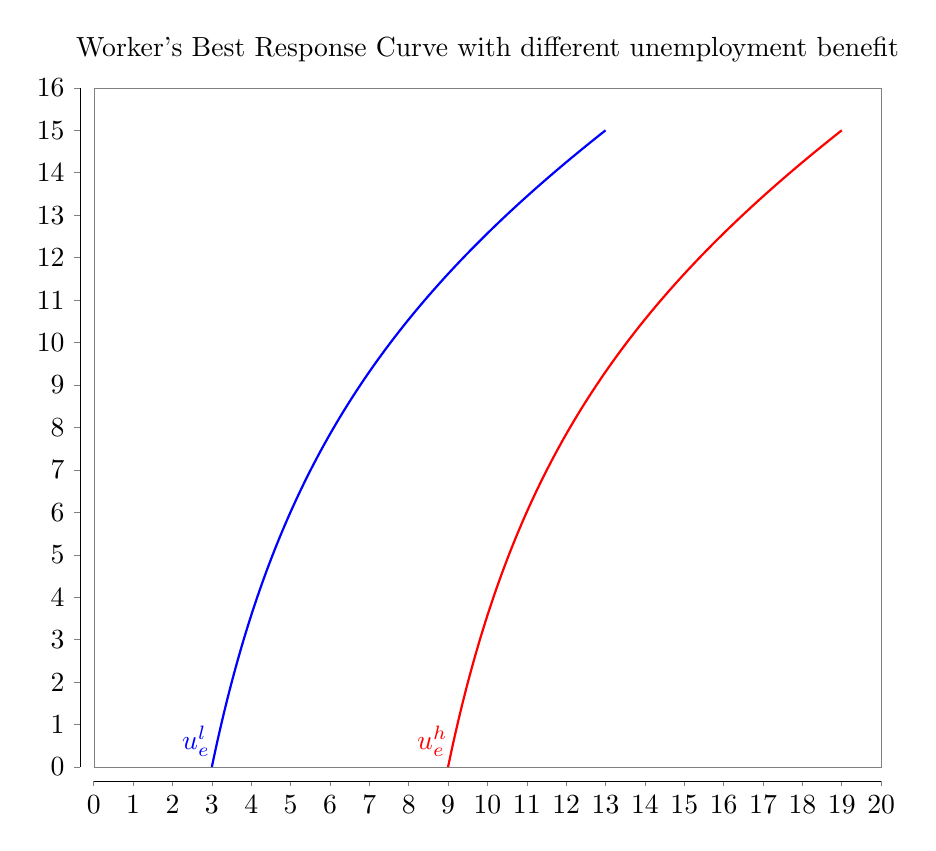
\begin{tikzpicture}

\begin{axis}[sciclean, xmin = 0, xmax = 20, ymin = 0, ymax = 16, title = {Worker's Best Response Curve with different unemployment benefit}]

\draw[thick, blue] (3, 0) node[above, xshift = -0.2cm]{$u_{e}^{l}$} to[bend left = 20] (13, 15);
\draw[thick, red, xshift = 3cm] (3, 0) node[above, xshift = -0.2cm]{$u_{e}^{h}$} to[bend left = 20] (13, 15);

\end{axis}

    % We could control parts of figure only shown in beamer or vice versa.
    % \ifstandalone
    %     \node[below=1cm of mid] {Only Shown in Standalone Figure};
    % \else
    %     \node[below=1cm of mid] {Only Shown in Beamer};
    % \fi
\end{tikzpicture}

\end{document}
